\documentclass[12pt,letterpaper]{article}
\usepackage[utf8]{inputenc}
\usepackage{amsmath}
\usepackage{amsfonts}
\usepackage{amssymb}
\usepackage{fancyhdr}
\usepackage{graphicx}
\usepackage[left=0.79in, right=0.79in, top=0.79in, bottom=0.79in]{geometry}
\usepackage{listings}
\usepackage{parskip}
\usepackage{subcaption}
\usepackage[svgnames]{xcolor}
\author{Chathan Driehuys}

\definecolor{diffstart}{named}{Grey}
\definecolor{diffincl}{named}{Green}
\definecolor{diffrem}{named}{OrangeRed}

\lstset{frame=tb,
	language=html,
	aboveskip=3mm,
	belowskip=3mm,
	showstringspaces=false,
	columns=flexible,
	basicstyle={\small\ttfamily},
	breaklines=true,
	breakatwhitespace=true,
	tabsize=2
}

\graphicspath{{./images/}}

\pagestyle{fancy}
\lhead{COMP 535}
\chead{Firewall}
\rhead{Chathan Driehuys}

\begin{document}
	\noindent \textbf{UNC Honor Pledge:} I certify that no unauthorized assistance has been received or given in the completion of this work.
	
	\vspace{.5in}
	
	\section*{Prerequisites}
		In order to demonstrate the effect of firewalls, we first had to set up two virtual machines (VMs) on the same network. To prove that the two machines can exchange traffic, we can ping one machine from another.
		
		\begin{figure}[h]
			\begin{center}
				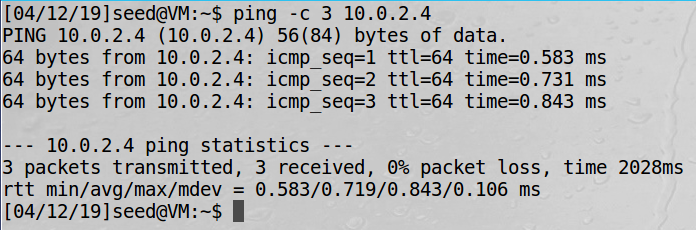
\includegraphics[width=4in]{task-0-ping}
			\end{center}
			\caption{The result of pinging one virtual machine from another.}
			\label{fig:task-0-ping}
		\end{figure}
	
	\section*{Task 1}
		Using the set of rules shown in Figure \ref{fig:task-1-ufw-rules}, we can block the following operations:
		
		\begin{enumerate}
			\item Telnet from A to B
			\item Telnet from B to A
			\item Access to \texttt{example.com} from A
		\end{enumerate}
		
		\begin{figure}
			\begin{center}
				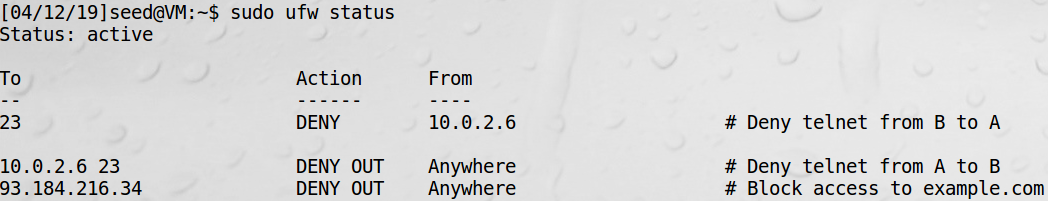
\includegraphics[width=\linewidth]{task-1-ufw-rules}
			\end{center}
			\caption{The \texttt{ufw} rules for task 1.}
			\label{fig:task-1-ufw-rules}
		\end{figure}
	
		In order to block traffic to \texttt{example.com} we must have an IP address to block. We can find that using the command \texttt{dig A example.com}. For images that show the result of adding the preceding rules, see Figures \ref{fig:task-1-telnet-a-b}, \ref{fig:task-1-telnet-b-a}, and \ref{fig:task-1-example-com}.
		
		\begin{figure}[p]
			\centering
			\begin{subfigure}{.5\linewidth}
				\centering
				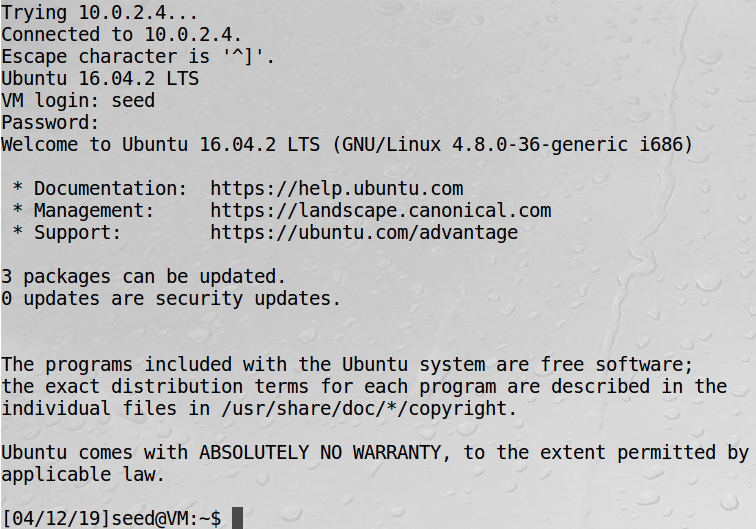
\includegraphics[width=.95\linewidth]{task-1-a-b-telnet-working}
			\end{subfigure}%
			\begin{subfigure}{.5\linewidth}
				\centering
				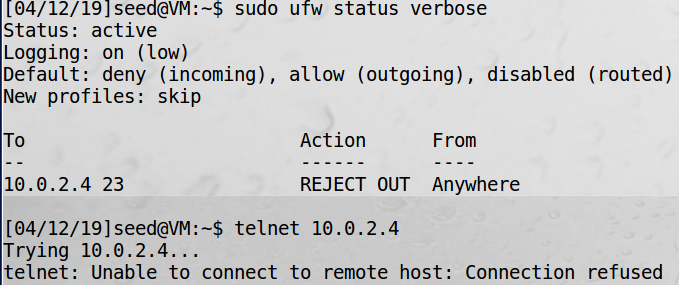
\includegraphics[width=.95\linewidth]{task-1-a-b-telnet-blocked}
			\end{subfigure}
			\caption{The Telnet connection from A to B that was previously working is now blocked.}
			\label{fig:task-1-telnet-a-b}
		\end{figure}
	
		\begin{figure}[p]
			\centering
			\begin{subfigure}{.5\linewidth}
				\centering
				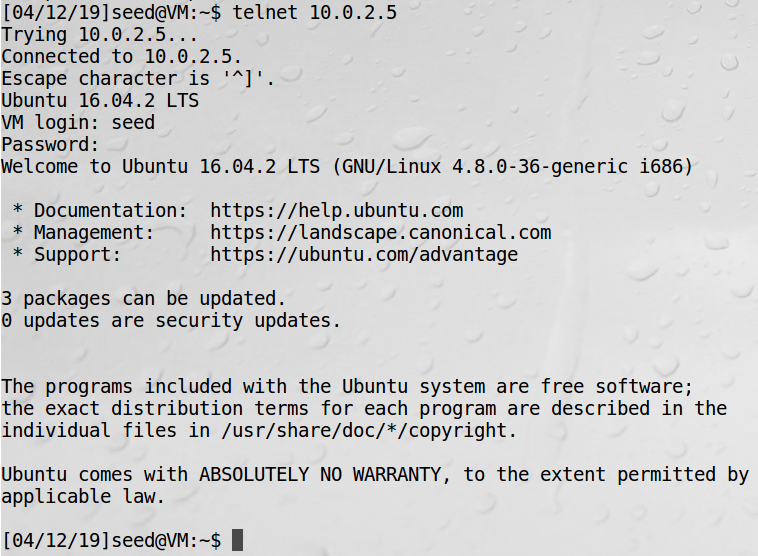
\includegraphics[width=.95\linewidth]{task-1-b-a-telnet-working}
			\end{subfigure}%
			\begin{subfigure}{.5\linewidth}
				\centering
				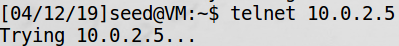
\includegraphics[width=.95\linewidth]{task-1-b-a-telnet-blocked}
			\end{subfigure}
			\caption{The Telnet connection from B to A that was previously working is now blocked.}
			\label{fig:task-1-telnet-b-a}
		\end{figure}
	
		\begin{figure}[p]
			\centering
			\begin{subfigure}{.5\linewidth}
				\centering
				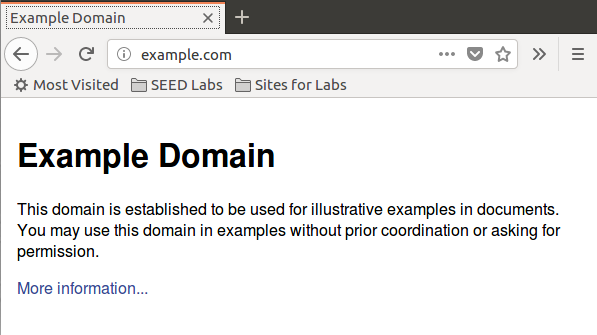
\includegraphics[width=.95\linewidth]{task-1-example-com-working}
			\end{subfigure}%
			\begin{subfigure}{.5\linewidth}
				\centering
				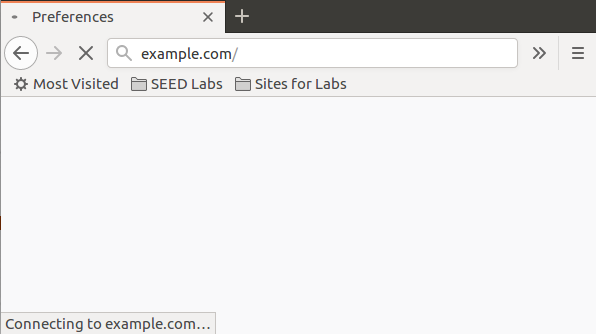
\includegraphics[width=.95\linewidth]{task-1-example-com-blocked}
			\end{subfigure}
			\caption{Access to \texttt{example.com} that was previously working is now blocked.}
			\label{fig:task-1-example-com}
		\end{figure}
	
	\section*{Task 2}
		In addition to the filters from the first task, we also implemented the following rules:
		
		\begin{enumerate}
			\item Block access to \texttt{syr.edu} from A
			\item Block SSH access from B to A
		\end{enumerate}
	
		Given the template for our firewall LKM from the lab instructions, we can add the following code to the pre or post routing hook to extract some useful information about each incoming or outgoing packet.
	
		\begin{lstlisting}[caption={Extracting info from packets.}, language=c]
struct iphdr *packet_header = (struct iphdr*) sk_network_header(skb);

// Our rules only apply to traffic using TCP.
if (ip_header->protocol == TCP_PROTO) {
	struct tcphdr *tcp_header = (struct tcphdr*) skb_transport_header(skb);
	
	unsigned int src_ip = (unsigned int) ip_header->saddr;
	unsigned int src_port = (unsigned int) ntohs(tcp_header->source);
	unsigned int dest_ip = (unsigned int) ip_header->daddr;
	unsigned int dest_port = (unsigned int) ntohs(tcp_header->dest);
}
		\end{lstlisting}
		
		Now that we have this information, it is fairly trivial to drop packets that meet specific criteria. For example, to implement the dropping of inbound telnet packets from machine B to machine A, we would add the following code to the hook for \texttt{NF\_INET\_PRE\_ROUTING}:
		
		\begin{lstlisting}[caption={Blocking telnet traffic from machine B to machine A}]
if (src_ip == MACHINE_B_IP) && dest_port == TELNET_PORT) {
	return NF_DROP;
}
		\end{lstlisting}
		
		All the implemented rules are variations of the above code sample that inspect various combinations of the source and destination IP address and port. For images showing the result of our firewall, see Figure~\ref{fig:task-2-results}.
		
		\begin{figure}[p]
			\begin{subfigure}{\linewidth}
				\centering
				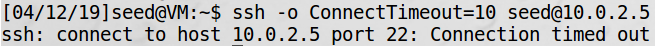
\includegraphics[width=4in]{task-2-ssh-timeout}
				\caption{An SSH connection from Machine B to Machine A timing out.}
				\label{fig:task-2-ssh-timeout}
			\end{subfigure}
		
			\vspace{.25in}
			
			\begin{subfigure}{\linewidth}
				\centering
				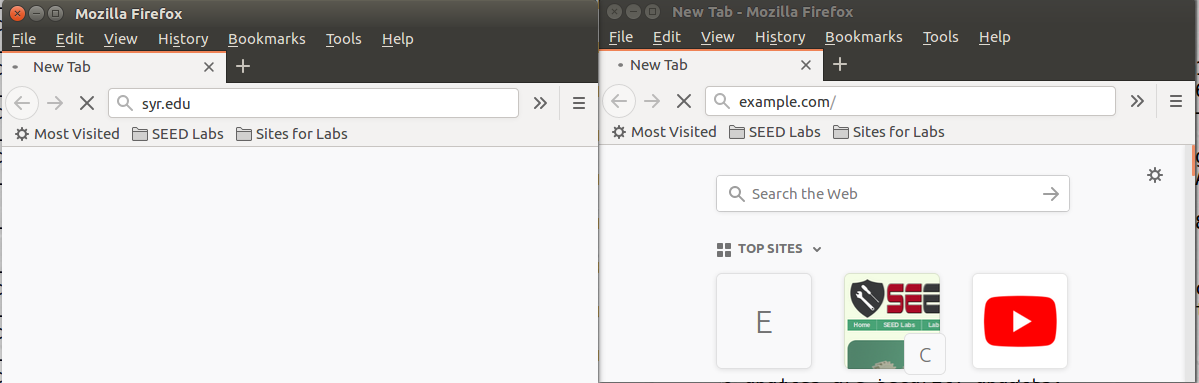
\includegraphics[width=\linewidth]{task-2-websites-blocked}
				\caption{Examples of blocked websites not loading.}
				\label{fig:task-2-websites-blocked}
			\end{subfigure}
		
			\caption{The result of our custom firewall}
			\label{fig:task-2-results}
		\end{figure}
	
	\pagebreak
		
	\section*{Task 3}
		The \texttt{ufw} rules for this task are show in Figure \ref{fig:task-3-ufw-rules}. They block any outgoing telnet connections from Machine A and any connections to Facebook from Machine A.
		
		\begin{figure}
			\begin{center}
				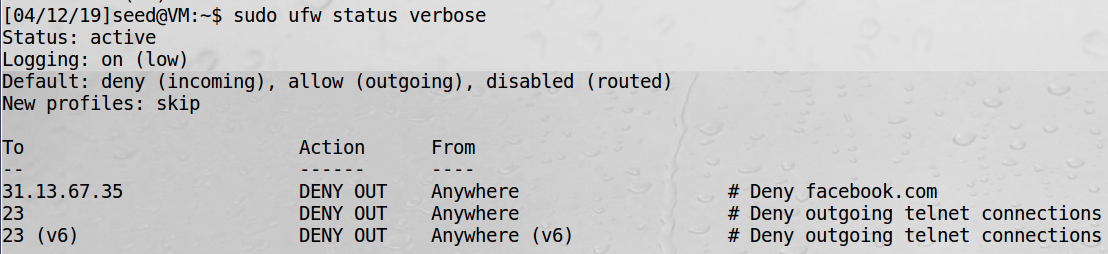
\includegraphics[width=\linewidth]{task-3-ufw-rules}
			\end{center}
			\caption{The \texttt{ufw} rules used to enable the filtering for Task 3}
			\label{fig:task-3-ufw-rules}
		\end{figure}
	
		\subsection*{Task 3.a}
			Assuming Machine B has the IP \texttt{10.0.2.5}, we can SSH tunnel into Machine B with:
			
			\begin{verbatim}
				ssh -L 8000:10.0.2.5:23 seed@10.0.2.5
			\end{verbatim}
			
			From this session, we can now telnet into Machine B on the tunnel we just opened using:
			
			\begin{verbatim}
				telnet localhost 8000
			\end{verbatim}
			
			This bypasses the filters set on Machine A because the packets are actually first being sent through an encrypted SSH connection to Machine B before being routed to their final destination. Since the firewall on Machine A has no rule prohibiting SSH traffic, this connection is allowed.
			
			Inspecting the packets that are being sent in this scenario reveals that the headers are consistent with a typical SSH connection. This is important because most firewalls use these headers to perform their filtering. Even if the firewall was inspecting the data within each packet (which is very performance intensive) it would not be able to detect anything since SSH traffic is encrypted.
			
		\subsection*{Task 3.b}
			After we set up the tunnel, we can connect to Facebook. Breaking the SSH tunnel and reloading Facebook fails with an error message that the socket is not accepting connections. If we disable the socket in Firefox, we now get an eternal loading page when attempting to navigate to Facebook because all the packets are being dropped. Enabling the socket again causes Facebook to load correctly.
			
			Similarly to the previous task, this works because the traffic leaving Machine A does not appear to the firewall to be destined for Facebook, which is blocked, but rather for Machine B over port 22. Once it has reached Machine B, the traffic is then routed to its actual destination of Facebook which is successful because Machine B has no firewall restrictions. The traffic returning from Facebook to Machine A is also not detected (or detectable) because the packets first return to Machine B and then travel back to Machine A through the SSH tunnel which is indistinguishable from any other (legitimate) SSH connection.
			
			Inspecting the packets that are being sent in this scenario reveals that the headers are consistent with a typical SSH connection. This is important because most firewalls use these headers to perform their filtering. Even if the firewall was inspecting the data within each packet (which is very performance intensive) it would not be able to detect anything since SSH traffic is encrypted.
			
	\section*{Task 4}
		As stated in the lab description, Machine B cannot access the web server or create an SSH connection to Machine A. The set of rules that accomplish that are shown in Figure \ref{fig:task-4-ufw-rules}. In this specific scenario, Machine A has the IP address \texttt{10.0.2.5} and Machine B has the IP address {10.0.2.6}.
		
		\begin{figure}[h]
			\begin{center}
				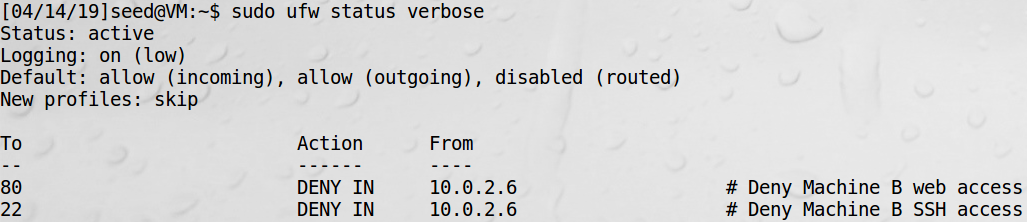
\includegraphics[width=\linewidth]{task-4-ufw-rules}
			\end{center}
			\caption{The \texttt{ufw} rules for task 4.}
			\label{fig:task-4-ufw-rules}
		\end{figure}
	
		In order to get around this ingress filtering, we can establish a reverse SSH tunnel from Machine A to Machine B that can grants Machine B access to the web server running on Machine A.
		
		\begin{verbatim}
			ssh -R 8080:localhost:80 seed@10.0.2.6
		\end{verbatim}
		
		The above command creates a tunnel on Machine B (\texttt{10.0.2.6}) accessible over port \texttt{8080} that forwards traffic to port \texttt{80} on Machine A (\texttt{localhost}).
		
		We can now visit \texttt{http://localhost:8080} in a browser on Machine B as seen in Figure~\ref{fig:task-4-web-access}.
		
		\begin{figure}[h]
			\begin{center}
				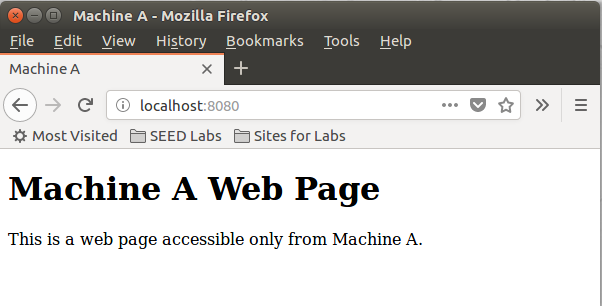
\includegraphics[width=4in]{task-4-web-access}
			\end{center}
			\caption{Accessing a web page through an SSH tunnel.}
			\label{fig:task-4-web-access}
		\end{figure}
\end{document}